\documentclass[onecolumn]{article}
\usepackage{graphicx} % Required for inserting images
\usepackage{amsmath}
\usepackage{amsfonts}
\usepackage{pythonhighlight}
\usepackage{datetime}
\usepackage{subcaption}
\usepackage{float}
\usepackage{titling}
\usepackage{enumitem}
\usepackage{matlab-prettifier}
\usepackage[colorlinks]{hyperref}
\usepackage[a4paper, total={6in, 8in}]{geometry}


\makeatletter
\Hy@AtBeginDocument{%
  \def\@pdfborder{0 0 1}% Overrides border definition set with colorlinks=true
  \def\@pdfborderstyle{/S/U/W 1}% Overrides border style set with colorlinks=true
                                % Hyperlink border style will be underline of width 1pt
}
\makeatother

\hypersetup{%
  colorlinks=true,
  linkcolor=blue,
  linkbordercolor=blue,% 
}
\footskip = 1pt
\textheight = 700pt
\setlength{\droptitle}{-10em}

\title{IN3170 V24 - Lab 3}
\author{Andreas Engøy, Simen Norrud, Erik Røset \& Daniel Tran}
\date{\monthname[\the\month] \the\year}

\begin{document}
\maketitle


\section{Task 1}
\subsection{Equipment}
\begin{table}[h]
    \centering
    \begin{tabular}{|c|c|c|}
        \hline
        \textbf{Component} & \textbf{Model} & \textbf{Quantity} \\
        \hline
        Resistor & 120k$\Omega$ & 1 \\
        Capacitor & 390pF & 6 \\
        Hex inverter & IC CD4007UBE & 2 \\
        Oscilloscope & HP54622 & 1 \\
        Waveform generator  & HP33120 & 1\\
        Voltage source & HPE3631 & 1 \\
        \hline
    \end{tabular}
    \caption{List of components used in task 1.}
    \label{tab:bom}
\end{table}

\subsection{Objective}
The objective of this task is to build two similar current source circuits, one with a CG current conveyor and one without, and observe the voltage discharge of the capacitor when the clock signal of the pFET transistors M2 goes low.  

\subsection{Theory}


\subsection{Constructing the circuits}

\begin{figure}[H]
    \centering
    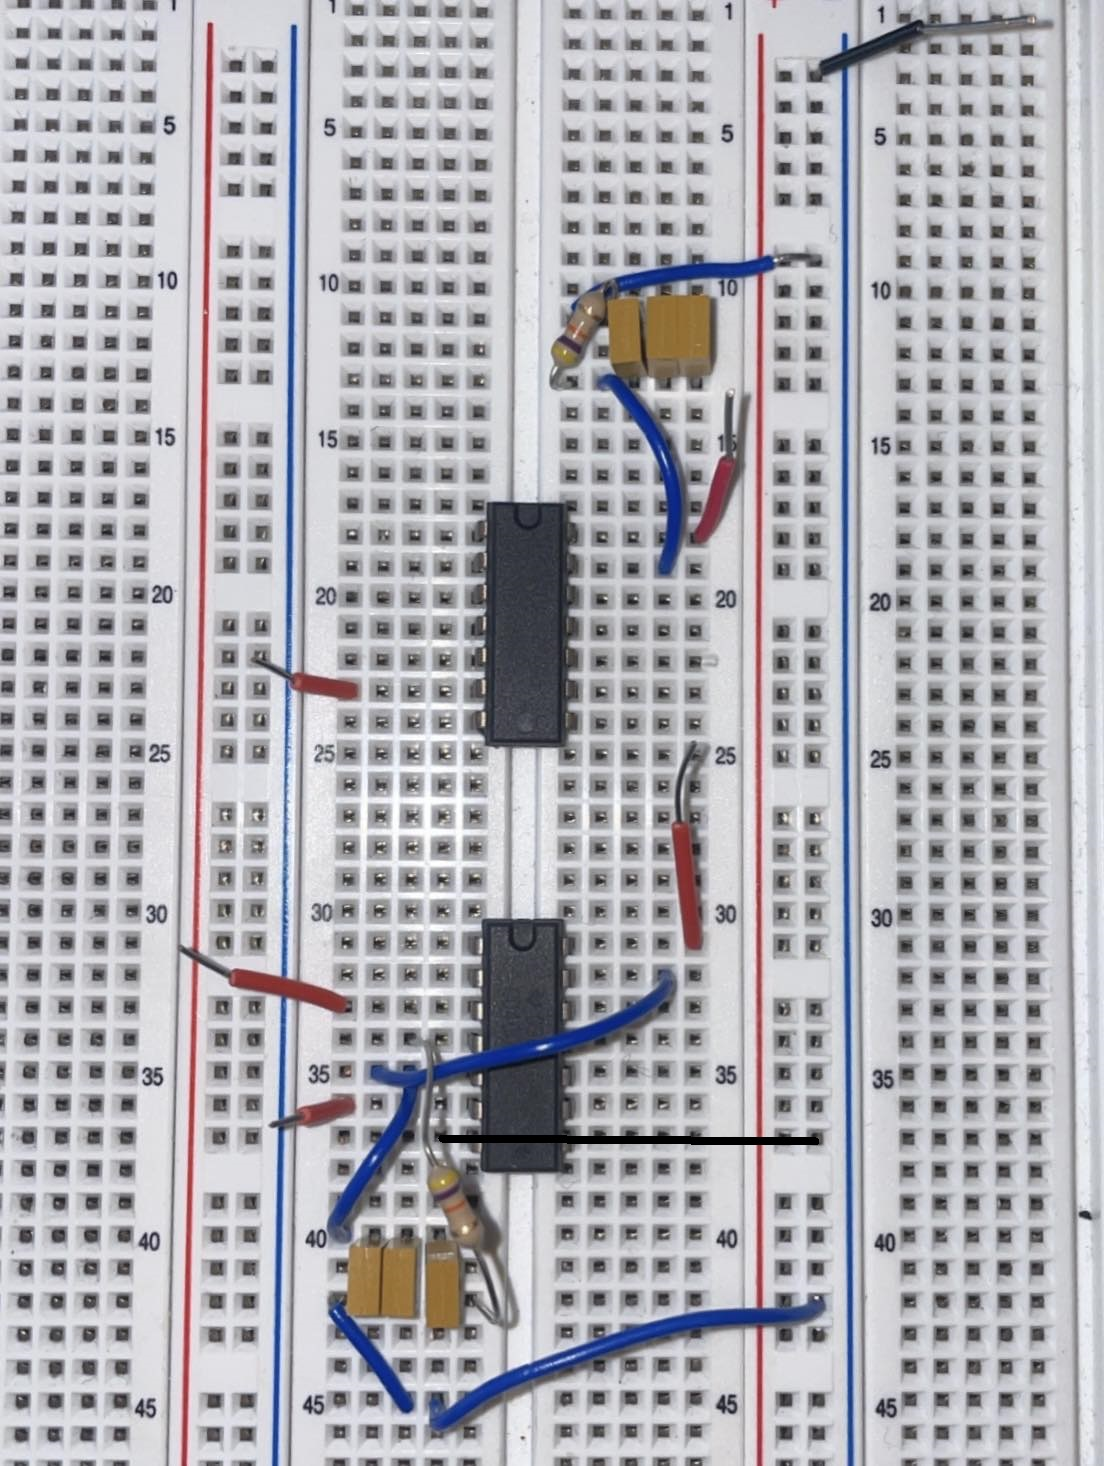
\includegraphics[scale=0.5]{LAB3/in3170lab3task1circuit.jpg}
    \caption{The two current source circuits used}
    \label{fig:enter-label}
\end{figure}

First, we will recreate the circuit from Figure 1 a) in the lab manual. Using the IC CD4007UBE we connected pin 14 to our $V_{DD}$ of 5V so as to give voltage to the Q1 pFET and the bulk of the pFETs. We connect pin 13, the source for pFETs, to the resistor and capacitors in parallel, and then to GND. Here we have replaced the $100k\Omega$ resistor with a $120k\Omega$. And the $1\mu F$ capacitor with three $390pF$ capacitors in parallel, totaling to $1.17nF$. This difference is significant as it is approximately three orders of magnitude less than the initial design value. Then, through the gate at pin 6, we connect a $5V_{pp}$ CLK signal.

To make the circuit from Figure 1 b) in the lab manual, connect the $V_{DD}$ to pin 14. Pin 13 is connected to the Q2 nFET through the drain at pin 5, the source at pin 4 is connected to the $120K\Omega$ resistor and further to GND. We apply a voltage ($V_{bias\_cascode}$) to the nFET at the pin 3 gate. Pin 13 is also connected to the capacitors, forming a parallel with the resistor and nFET, and then connected to GND. Then, connect the Q1 gate at pin 6 to the CLK signal and pin 7, the bulk of the nFETs, to GND.

The voltage on C would be a constant voltage, as the current source would be able to supply a constant current to the capacitor. The voltage on the capacitor would then be given by the formula $V = \frac{Q}{C}$, where $Q$ is the charge on the capacitor and $C$ is the capacitance of the capacitor. The charge on the capacitor is given by $Q = I \cdot t$, where $I$ is the current and $t$ is the time. As the current is constant, the charge on the capacitor will be linear with time, and the voltage on the capacitor will be linear with time.

As the 100k$\Omega$ resistor was not available at the lab we used a 120k$\Omega$ instead. As per lab instructions we calculated the current through the resitor at 1V to be 

\begin{align}
    I = \frac{V}{R} = \frac{1V}{120k\Omega} = 8.33\mu A
\end{align}

To get the discharge curve we used the $I = \frac{V}{dt}C$ relation to get the time it would take for the voltage to drop to 0V, which would be the time it takes for the capacitor to discharge through the resistor.

\begin{align}
    I = \frac{V}{dt}C \Rightarrow dt = \frac{V}{I} C = \frac{5V}{8.33\mu A}\cdot 3*0.39nF = 0.702ms
\end{align}

\begin{figure}[h!]
    \centering
    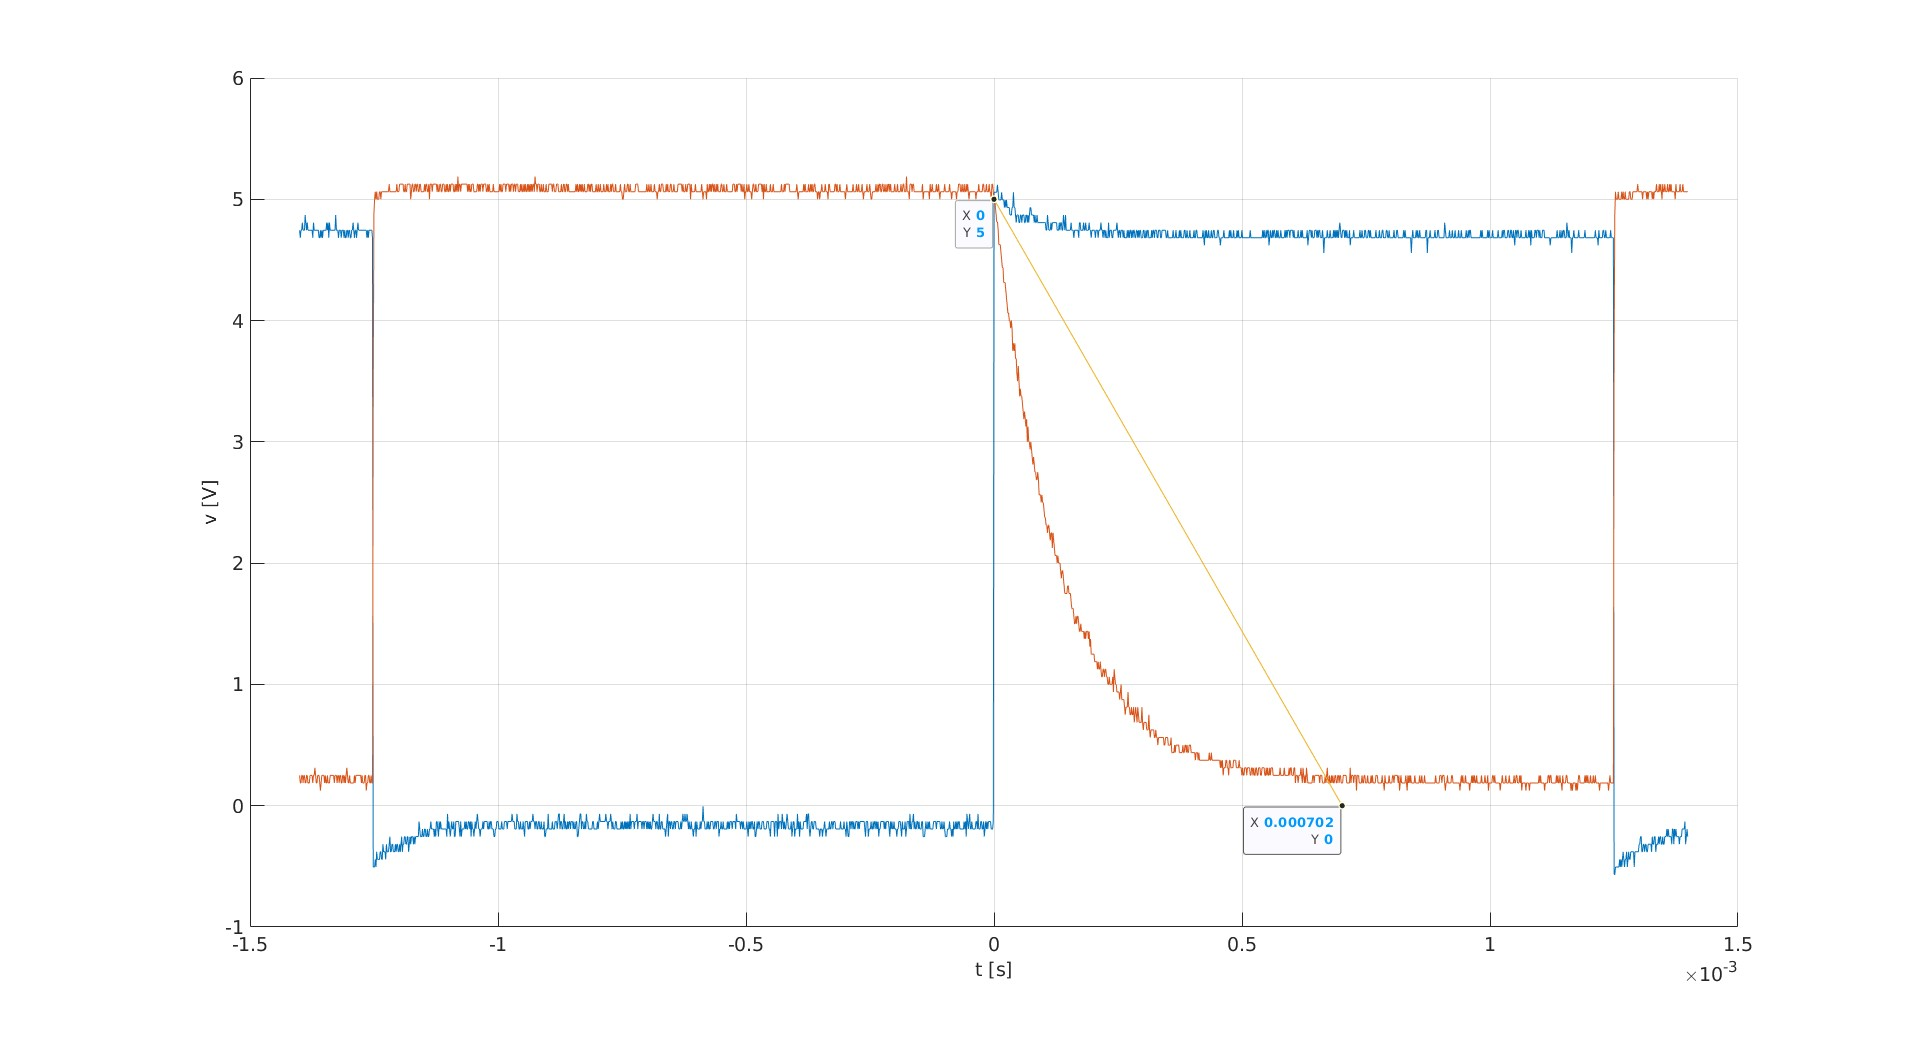
\includegraphics[width=0.7\textwidth]{1a.jpg}
    \caption{Plot of the circuit in figure 1 a) in the lab manual with the ideal discharge curve in yellow.}
    \label{fig:task1a}
\end{figure}

As seen in \ref{} the actual discharge curve is not linear, but rather exponential as per a capacitors normal discharge characteristics. This is due to the fact that M2s gate voltage is 0V when the clocked signal is low which gives a $|V_{GS}| \lt |V_{TH}|$, moving the pFET from saturation to cutoff. With no voltage at the gate, the pFET will not conduct any current, and the capacitor will discharge through the resistor. The voltage on the capacitor will then be given by $V = V_{DD} \cdot e^{-\frac{t}{RC}}$, where $R$ is the resistance and $C$ is the capacitance of the capacitor.

\begin{figure}[h!]
    \centering
    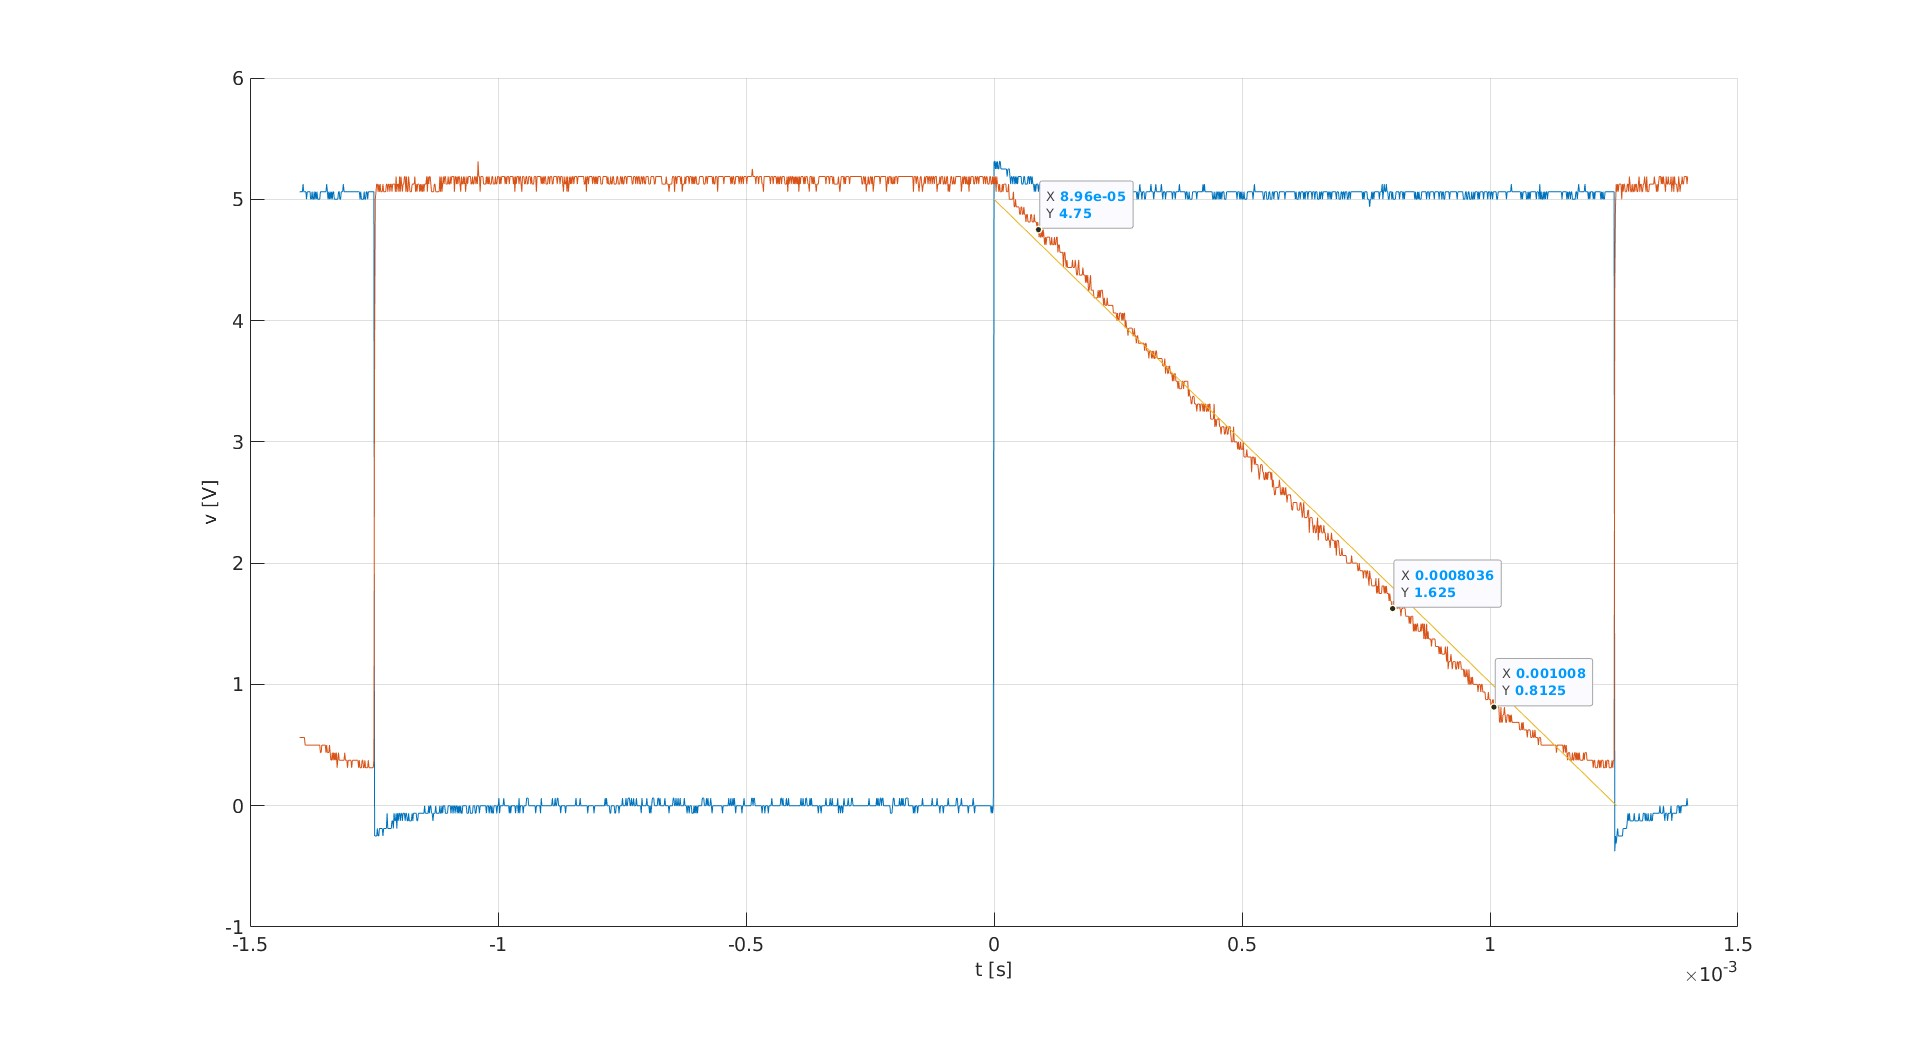
\includegraphics[width=0.7\textwidth]{1b.jpg}
    \caption{Plot of the circuit in figure 1 b) in the lab manual with the ideal discharge curve in yellow.}
    \label{fig:task1b}
\end{figure}

In stark contrast to the previous circuit, the circuit in \ref{fig:task1b} follows the theoretical curve down to what we observe to be around 1.2V when we apply 3V on the gate of M1. This is because of the relations $I_D$ and $V_{DS}$in saturation and triode region. We have that:

\begin{align}
    I_D = \frac{1}{2} \cdot \mu_n \cdot C_{ox} \cdot \frac{W}{L} \cdot (V_{GS} - V_{TH})^2(1 - \lambda \cdot V_{DS})
\end{align}

for the saturation region, aka when $V_{DS} \geq V_{GS} - V_{TH}$, and $V_{GS} \geq V_{TH}$. For the triode region, aka when $V_{DS} \lt V_{GS} - V_{TH}$, and $V_{GS} \geq V_{TH}$, we have that:

\begin{align}
    I_D = \mu_n \cdot C_{ox} \cdot \frac{W}{L} \cdot (V_{GS} - V_{TH} - \frac{V_{DS}}{2}) \cdot V_{DS}
\end{align}

From the equations above we can observe 

\section{Task 2}

\subsubsection*{Objective}
The objective of this task is to improve a current source using a FET in saturation. By simulating the circuit in Cadence one can plot the $I_D$ vs $V_{DS}$ curve and calculate the output resistance $r_{ds}$ of the current source. Further, changing the design parameter $\frac{W}{L}$ of the FET, or adding a voltage cascode to the circuit is carried out to improve the current source capability.

\subsection*{Theory}

In an ideal current source, the output current is independent of the voltage across the terminals. I.e. the current source maintains the same current throughout the circuit, despite changes to $V_{DS}$.

A Field-Effect Transistor (FET) operating in the saturation region exhibits the same characteristics as an ideal current source. This can be seen from the $I_D$ vs $V_{DS}$ curve in the saturation region, where the current is almost constant. This is because when  $V_{DS}$ approches the saturation region it becomes high enough that it maxes out the number of charge carriers that can contribute to current flow, making the gate voltage the primarily factor to the current flow.

In the plot, the curve will flatten out in this region. In a practical FET, the curve will not be completely flat (indicating that the current is not completely constant), but it will give a good approximation of an ideal current source.


 \clearpage

\subsubsection*{Designing a current source}

\begin{figure}[h!]
    \centering
    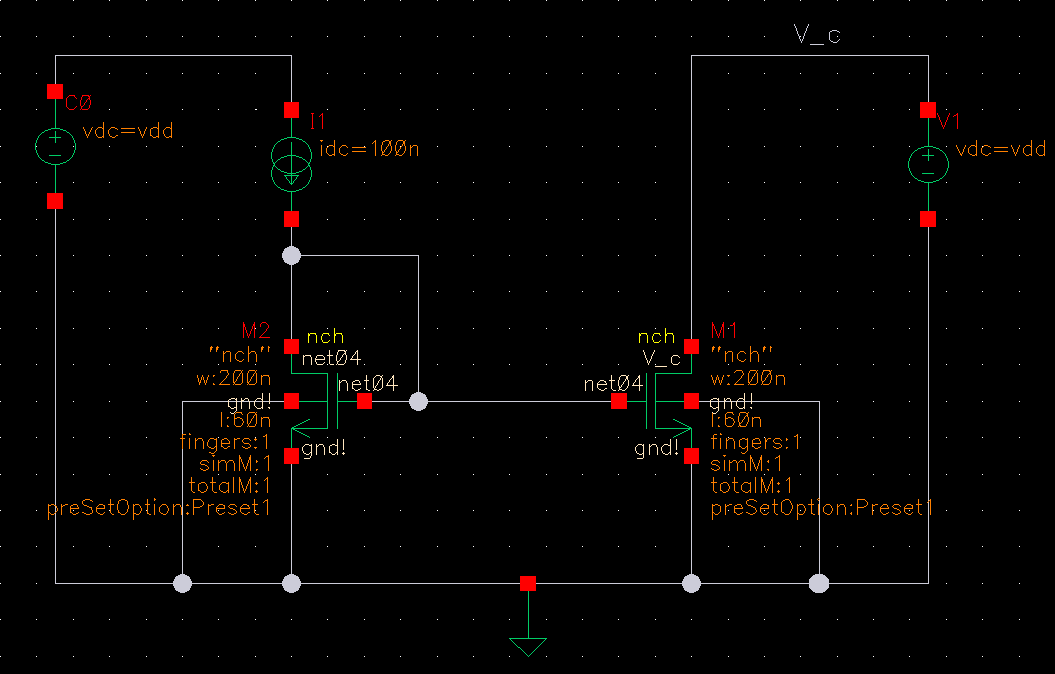
\includegraphics[width=1\textwidth]{circuit_c_fixed.png}
    \caption{Screencapture of the circuit in figure 1 c) from the lab manual simulated in Cadence.}
    \label{fig:circuitc}
\end{figure}

This design differs a bit from figure 1 d) in the lab manual, following the suggested method of the manual. The bias current is implementet as a current mirror, consisting of $M2$ and $I1$, which sets the current that flows through $M1$. Instead of a capactior in parallel to $M1$, and a clock signal to $M2$, a DC voltage source is used to sweep the voltage $V_C$ in a range simulating the $V_{DS}$ of $M1$. 

\clearpage 

\begin{figure}[h!]
    \centering
    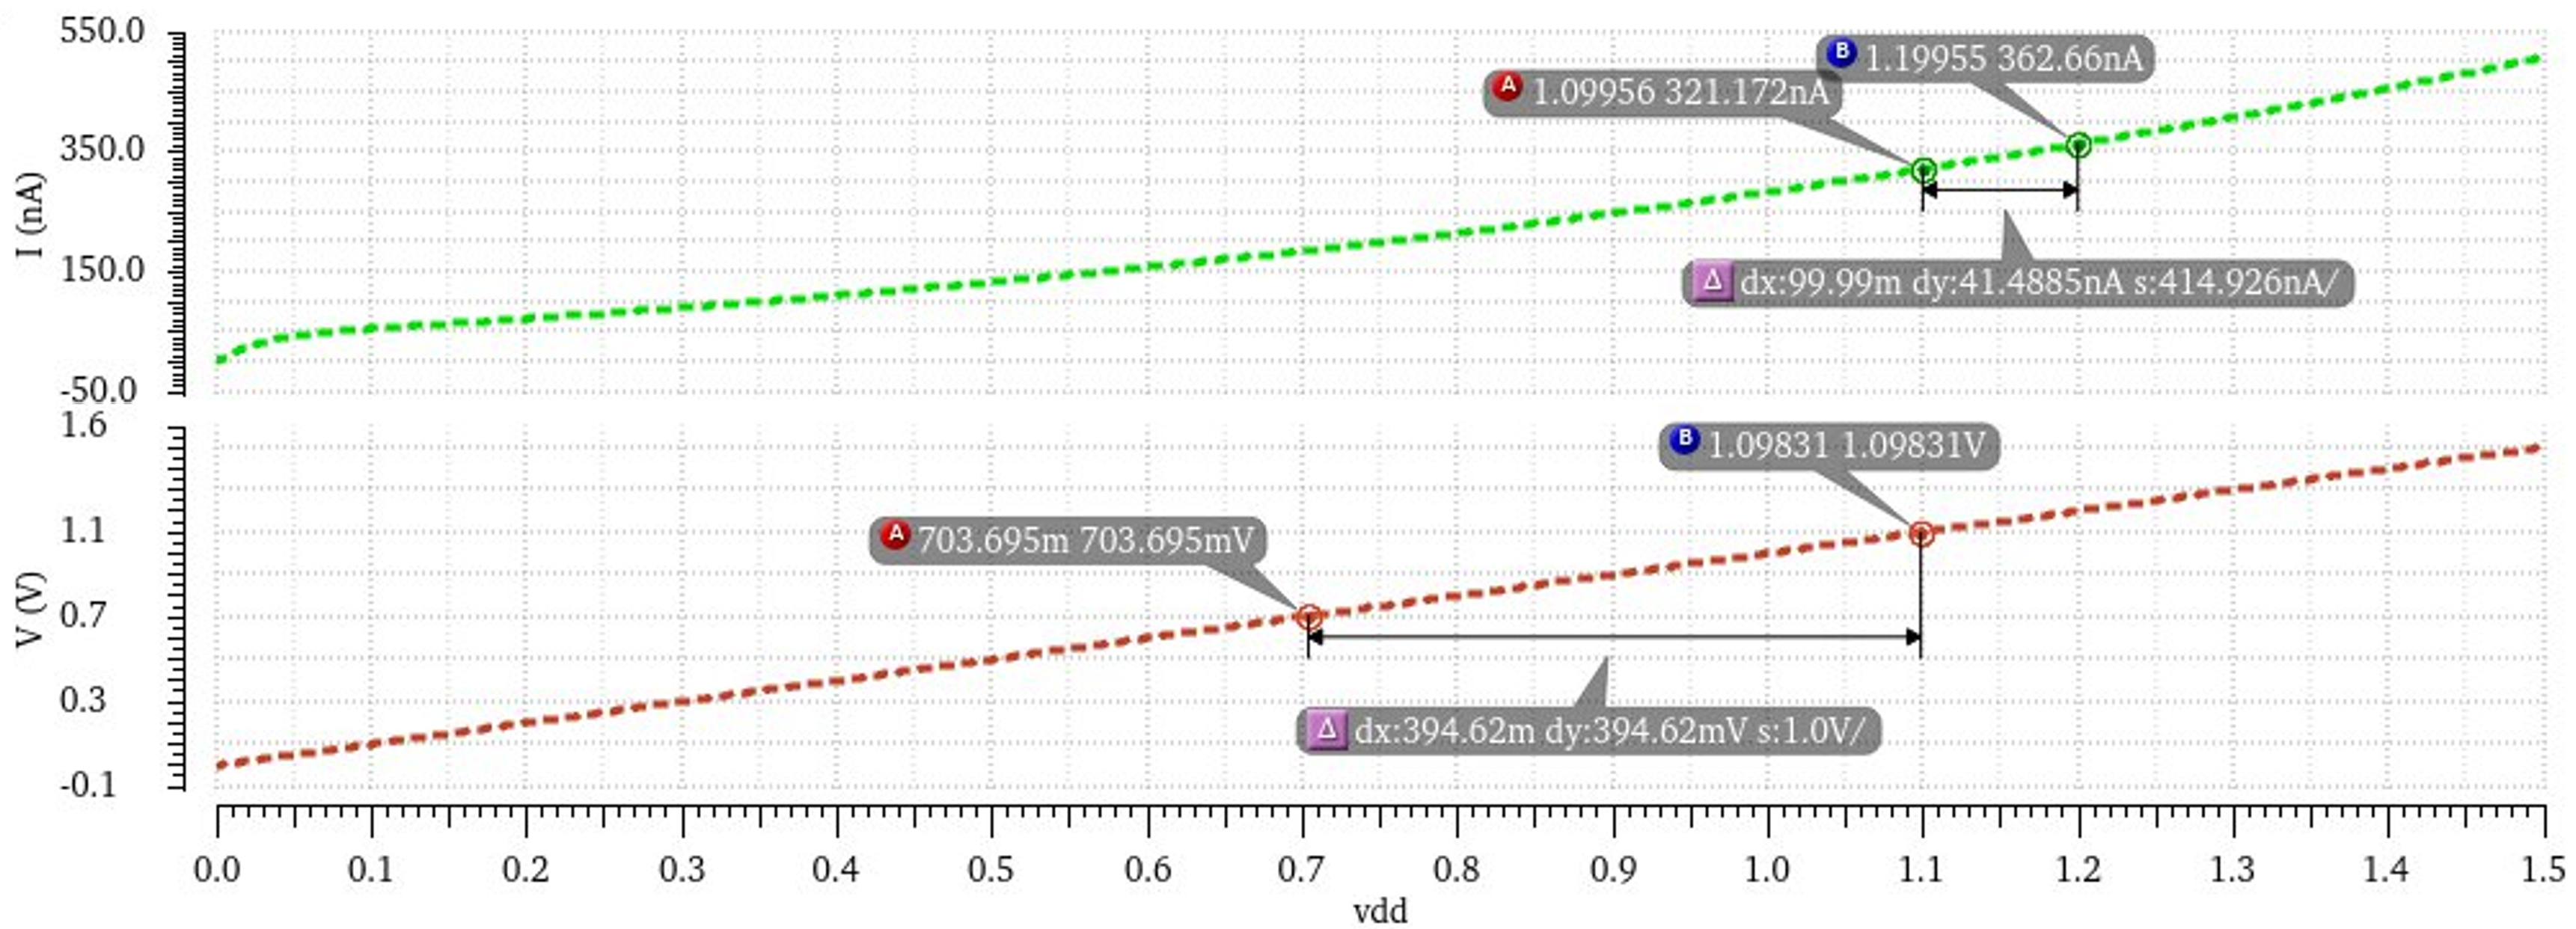
\includegraphics[width=1\textwidth]{plot_circuit_c_FINAL.png}
    \caption{Screencapture of the DC sweep of the circuit in figure 1.}
    \label{fig:plotc}
\end{figure}

$\Delta I_D$ is calculated as the difference between two points on the \textit{most linear} part of the curve. In figure \ref{fig:plotc}, this is chosen to be a segment at the end of the curve. The DC sweep simulation is set to sweep from $0 \ \text{V}$ to $1.5 \ \text{V}$. The lab manual specifies to use only up to $1.2 \ \text{V}$, hence the last point is chosen to be close up to $1.2 \ \text{V}$.
\begin{align}
    \Delta I_D &= 414.926 \ \text{nA}
\end{align}

The same method is used to calculate $\Delta V_{DS}$, however as $V_C$ is the sweep parameter, the voltage rises lineary. The difference between two points on this line will be the same wherever. In figure \ref{fig:plotc}, the points are chosen arbitrarily.

\begin{align}
    \Delta V_{DS} = 1 \ \text{V}
\end{align}
$r_{ds}$ can then simply be calculated using Ohm's Law:
\begin{align}
    r_{ds} = \frac{\Delta V_{DS}}{\Delta  I_D} = \frac{ 1 \ \text{V}}{414.926 \ \text{nA}} = 2.4007 \ \text{M}\Omega
\end{align}

The next task is to tinker with the design parameter $\frac{W}{L}$ of $M1$ in order to improve the current source capability. Even in saturation, real FETs exhibit channel-length modulation, which is a phenomenon where the effective channel length shortens as $V_{DS}$ increases, leading to a non-ideal increase in current. By increasing the channel length $L$ of the transistor, the channel-length modulation is reduced, and the current source capability is improved.
In this rapport the channel length was increased to $L = 1 \ \mu m$. This is an exaggeration of what a normal channel length would be, but will highlight the difference more. A DC sweep is then performed again, resulting in the following plot: 

\begin{figure}[h!]
    \centering
    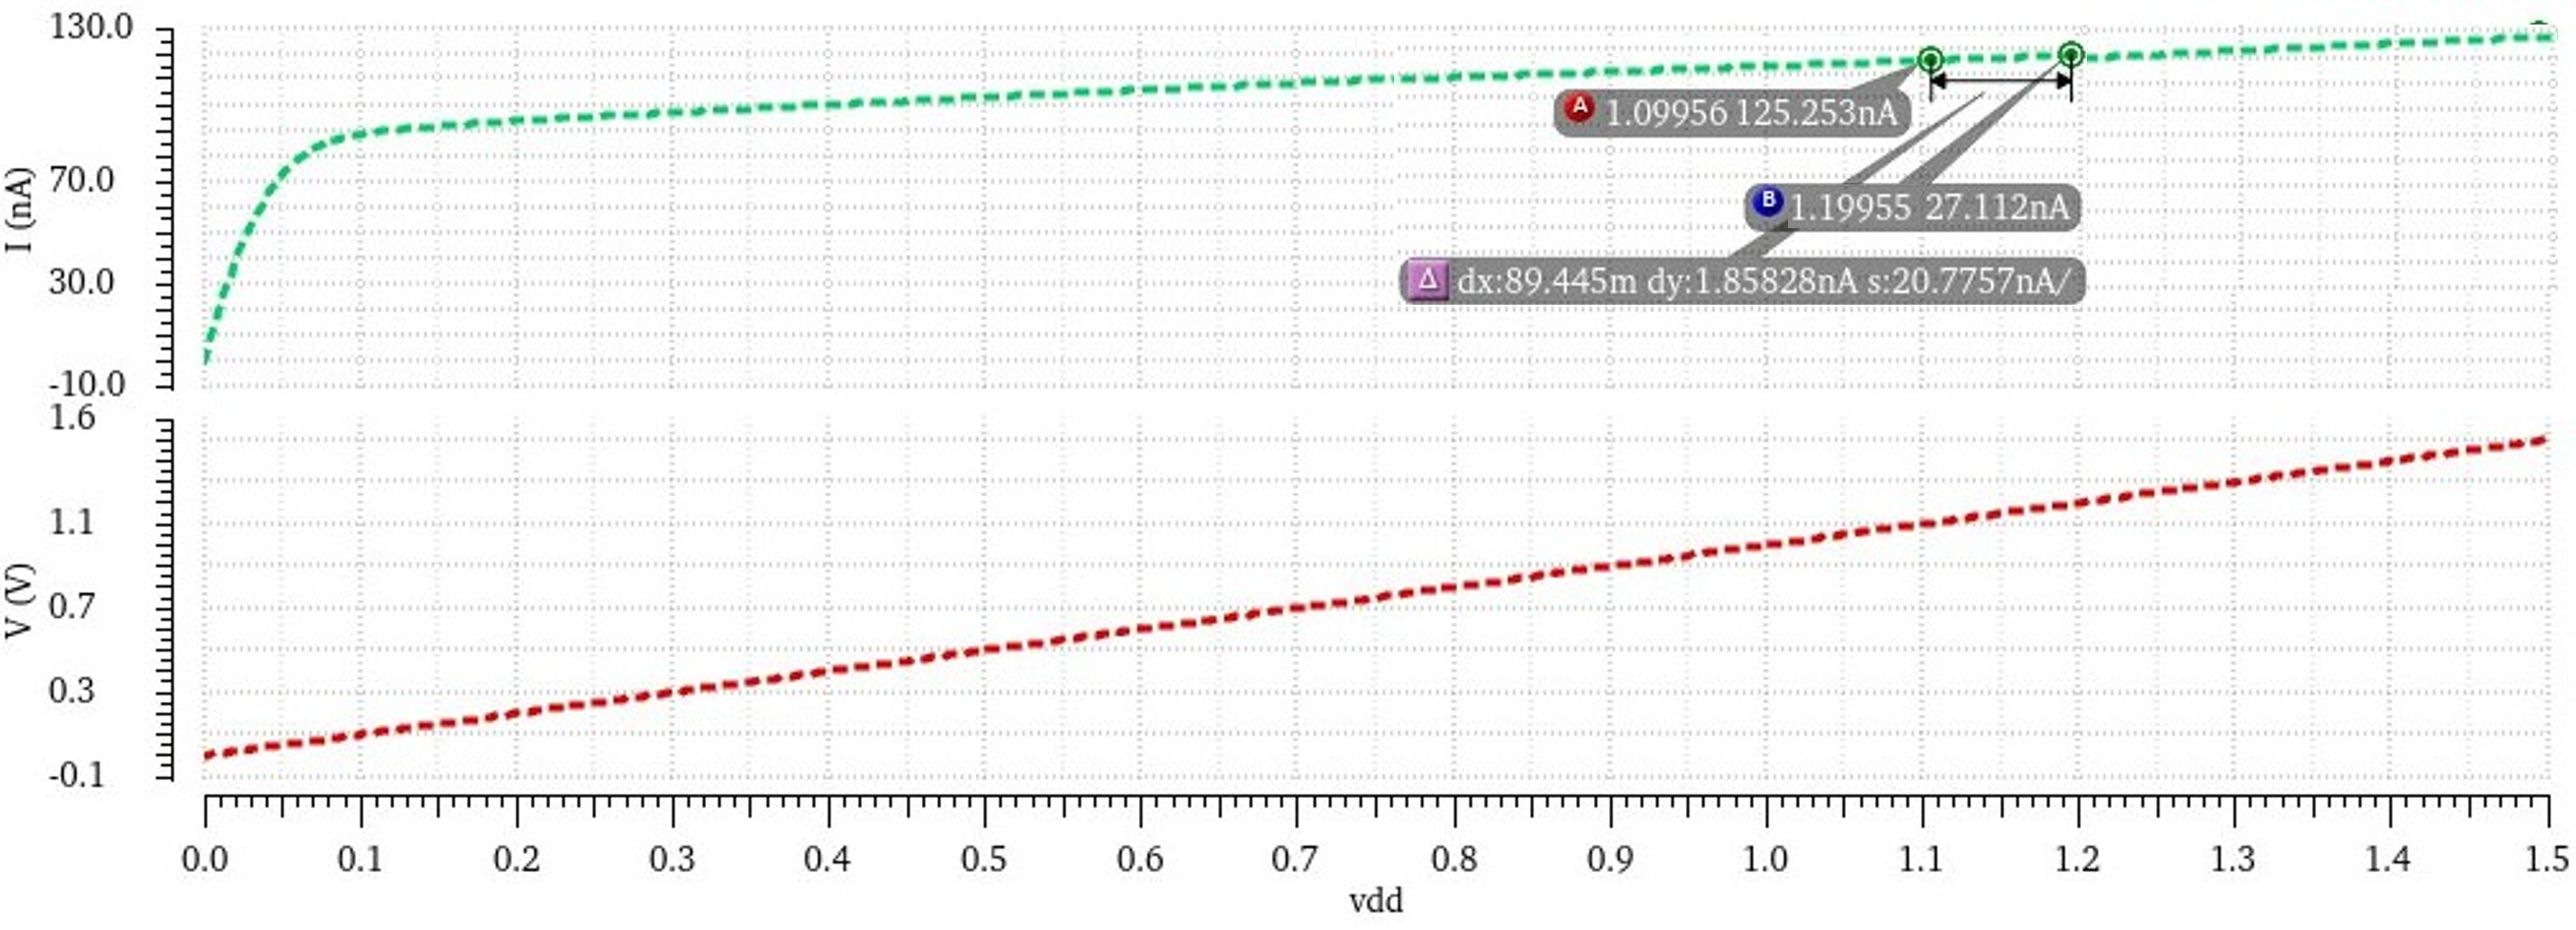
\includegraphics[width=1\textwidth]{plot_circuit_d_FINAL.png}
    \caption{Screencapture of the DC sweep of the circuit in figure 1 with $L = 1 \ \mu m$ for $M1$ and $M2$.}
    \label{fig:plotcnew}
\end{figure}

For the circuit in figure \ref{fig:plotcnew}, the same method is used to calculate $\Delta I_D$ and $\Delta V_{DS}$ as for the previous circuit. $r_{ds}$ is then:

\begin{align}
    r_{ds} = \frac{\Delta V_{DS}}{\Delta  I_D} = \frac{ 1 \ \text{V}}{20.7757 \ \text{nA}} = 4.8133 \ \text{M}\Omega
\end{align}


In a ideal current source, the output resistance (or $V_{ds}$) is infinite. The new $r_{ds}$ is higher than the previous, which indicates a better approximation of an ideal current source.

\clearpage

\subsubsection*{Implementing a voltage cascode}

\begin{figure}[h!]
    \centering
    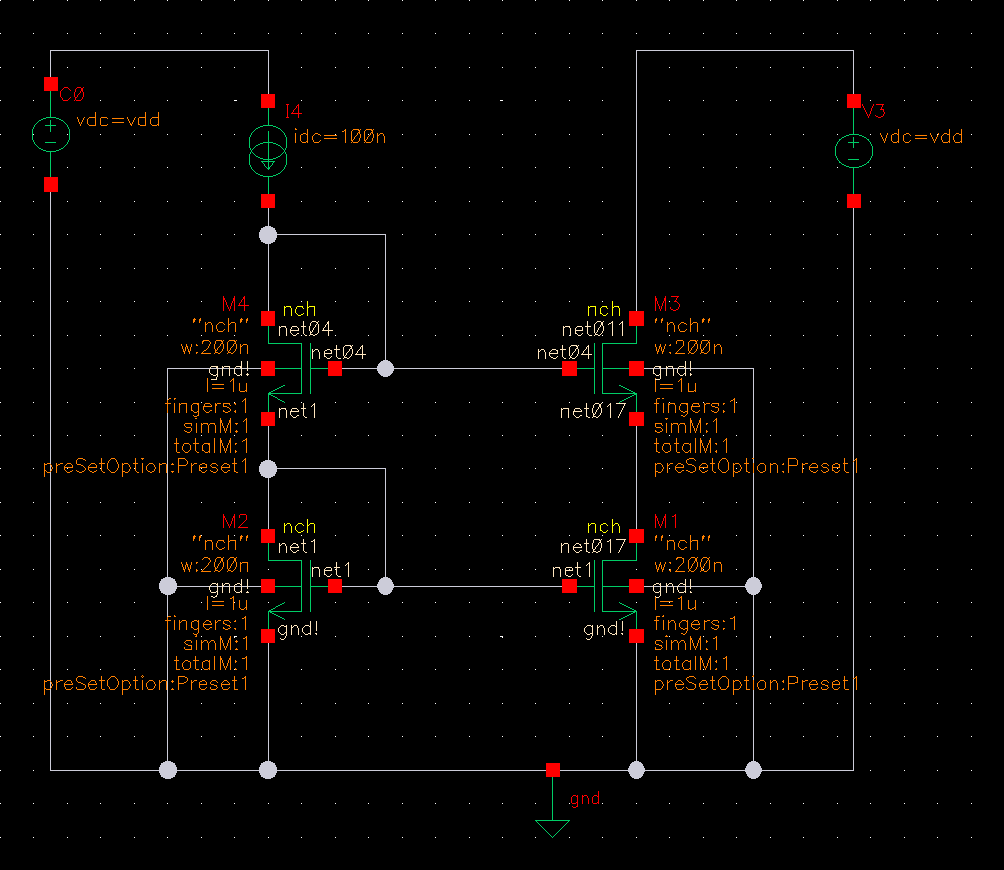
\includegraphics[width=0.7\textwidth]{circuit_d_cascode.png}
    \caption{Screencapture of the circuit in figure 1 d) from the lab manual simulated in Cadence.}
    \label{fig:circuitd}
\end{figure}

\begin{figure}[h!]
    \centering
    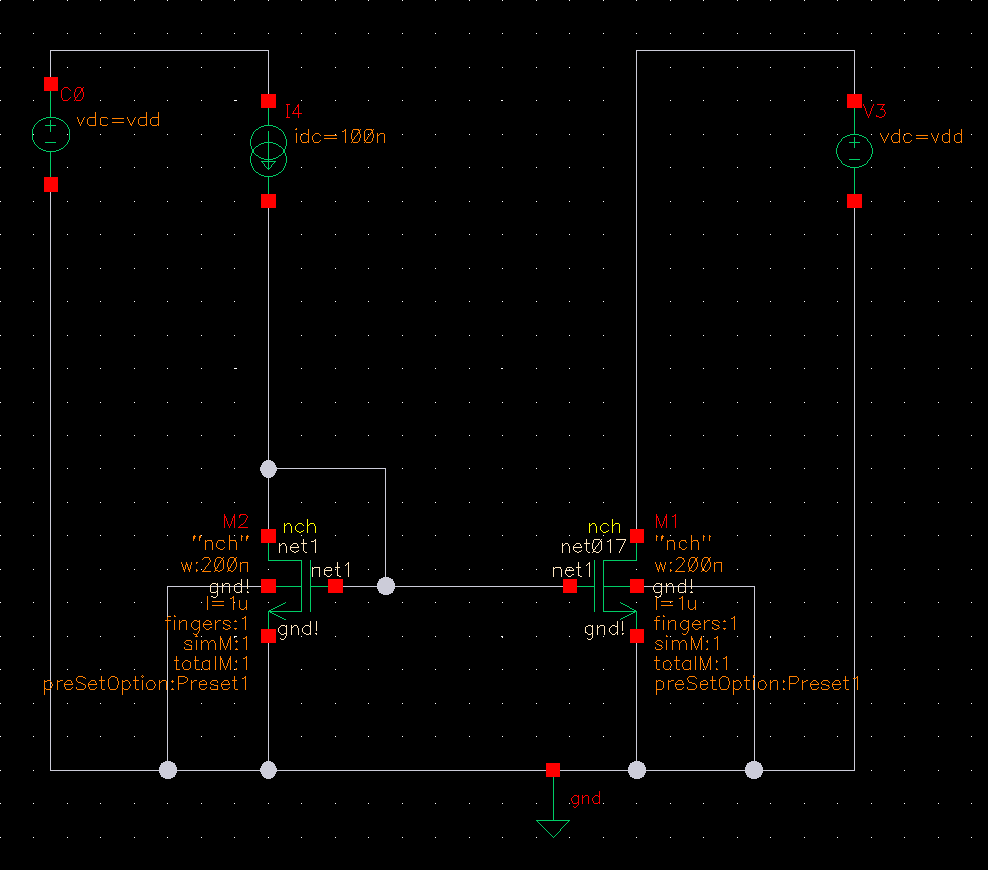
\includegraphics[width=0.7\textwidth]{circuit_d_simple.png}
    \caption{Screencapture of the circuit in figure 1 d) from the lab manual without the voltage cascode simulated in Cadence.}
    \label{fig:circuitdsimple}
\end{figure}

\clearpage

In similar fashion as the previous circuits, a DC sweep is performed for the circuit in figure \ref{fig:circuitd} and \ref{fig:circuitdsimple}:

\begin{figure}[h!]
    \centering
    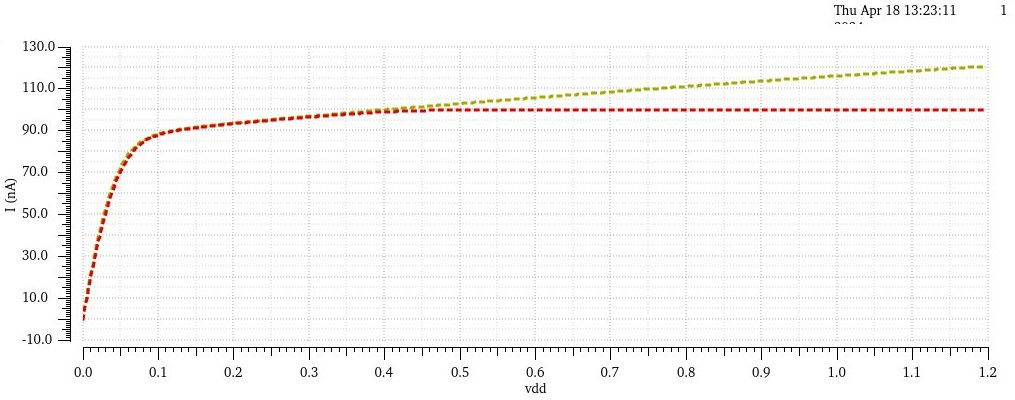
\includegraphics[width=1\textwidth]{plot_circuit_d_dc_sweep_omskjert.jpg}
    \caption{Screencapture of the DC sweep of both circuits in figure 1 d).}
    \label{fig:plotd}
\end{figure}

In figure \ref{fig:plotd}, the red curve is the simulated $I_D$ vs $V_{C}$ for the circuit in figure \ref{fig:circuitd}. The yellow curve is equivalent curve for the circuit in figure \ref{fig:circuitdsimple} plotted alongside for comparison.  

Initially one can observe the two curves starts off nearly identical. As $V_{C}$ increases, the current in both circuits begins with a sharp rise but starts to flatten as the transistors approach the saturation region. The cascode configuration, however, shows a distinct change in behavior around $0.4$ V where the current flattens out even more. This enhanced flattening is due to the cascode transistor $M3$, which further restricts the increase in current by also entering saturation and increasing the circuit's output impedance.

Some trade-offs associated with using a cascode configuration include a reduced voltage headroom. That is, the circuit requires a minimum voltage drop across each transistor to ensure that both are operating in saturation. Essentially, the drain-source voltage $V_{DS}$ of the cascode transistor $M3$ must be sufficiently high for it to remain in saturation. A cascode circuit also adds complexity to the system that might be unnecessary. If the applied voltage range is small, there will be no benefit to using a cascode configuration, as the cascode transistor will not enter saturation.

\end{document}